%!TEX program = xelatex
\documentclass[a4paper,12pt]{report}
\usepackage{ctex}
\usepackage{caption}%并排图片
\usepackage{subfigure}%并排图片
%\usepackage{xeCJK}{}
\usepackage{times}
\usepackage{setspace}
\usepackage{fancyhdr}
\usepackage{graphicx}
\usepackage{wrapfig}
\usepackage{array}  
\usepackage{fontspec,xunicode,xltxtra}
\usepackage{titlesec}
\usepackage{titletoc}
\usepackage[titletoc]{appendix}
\usepackage[top=30mm,bottom=30mm,left=20mm,right=20mm]{geometry}
\usepackage{cite}
\usepackage{listings}
\usepackage[framed,numbered,autolinebreaks,useliterate]{mcode} % 插入代码
\XeTeXlinebreaklocale "zh"
\XeTeXlinebreakskip = 0pt plus 1pt minus 0.1pt

%---------------------------------------------------------------------
%	页眉页脚设置
%---------------------------------------------------------------------
\fancypagestyle{plain}{
	\pagestyle{fancy}      %改变章节首页页眉
}

\pagestyle{fancy}
\lhead{\kaishu~Mask R-CNN报告~}
\rhead{\kaishu~173800801~沈天马~}
\cfoot{\thepage}

%---------------------------------------------------------------------
%	章节标题设置
%---------------------------------------------------------------------
\titleformat{\chapter}{\centering\zihao{-1}\heiti}{\chinese{chapter}}{1em}{}
\titlespacing{\chapter}{0pt}{*0}{*6}

%---------------------------------------------------------------------
%	摘要标题设置
%---------------------------------------------------------------------
\renewcommand{\abstractname}{\zihao{-3} 摘\quad 要}

%---------------------------------------------------------------------
%	参考文献设置
%---------------------------------------------------------------------
\renewcommand{\bibname}{\zihao{2}{\hspace{\fill}参\hspace{0.5em}考\hspace{0.5em}文\hspace{0.5em}献\hspace{\fill}}}

%---------------------------------------------------------------------
%	引用文献设置为上标
%---------------------------------------------------------------------
\makeatletter
\def\@cite#1#2{\textsuperscript{[{#1\if@tempswa , #2\fi}]}}
\makeatother

%---------------------------------------------------------------------
%	目录页设置
%---------------------------------------------------------------------
\titlecontents{chapter}[0em]{\songti\zihao{-4}}{\thecontentslabel\ }{}
{\hspace{.5em}\titlerule*[4pt]{$\cdot$}\contentspage}
\titlecontents{section}[2em]{\vspace{0.1\baselineskip}\songti\zihao{-4}}{\thecontentslabel\ }{}
{\hspace{.5em}\titlerule*[4pt]{$\cdot$}\contentspage}
\titlecontents{subsection}[4em]{\vspace{0.1\baselineskip}\songti\zihao{-4}}{\thecontentslabel\ }{}
{\hspace{.5em}\titlerule*[4pt]{$\cdot$}\contentspage}


\begin{document}
%---------------------------------------------------------------------
%	封面设置
%---------------------------------------------------------------------
\begin{titlepage}
	\begin{center}
		
    
\includegraphics[width=0.55\textwidth]{figure//Njust.png}\\
    \vspace{10mm}
    \textbf{\zihao{1}\kaishu{研究生课程(论文类)试卷}}\\[0.8cm]
    \textbf{\zihao{3}\kaishu{ \underline { 2016 }/\underline{ 2017 }学年第 \underline{ 1 } 学期}}\\[0.8cm]
    
	
\setlength{\extrarowheight}{1mm}
{\songti\zihao{3}	
\begin{tabular}{rl}
	
	{\makebox[4\ccwd][s]{\kaishu 课程名称:}}& ~\kaishu \underline { \quad \quad \quad 图像处理与分析 \quad \quad \quad \quad}\\[0.5cm]
	
	{\makebox[4\ccwd][s]{\kaishu 课程代码:}}& ~\kaishu \underline { \quad \quad \quad \quad \quad 12010048 \quad \quad \quad \quad \quad} \\ [0.5cm]

    {\makebox[4\ccwd][s]{\kaishu 论文题目:}}& ~\kaishu \underline { \quad \quad \quad \quad  Mask R-CNN \quad \quad \quad \quad } \\ [0.5cm]
   
	{\makebox[4\ccwd][s]{\kaishu 学生姓名:}} & ~\kaishu \underline { \quad \quad \quad \quad \quad  沈天马 \quad \quad \quad \quad \quad \quad }\\ [0.5cm]

	{\makebox[4\ccwd][s]{\kaishu 专业,学号:}} & ~\kaishu \underline { \quad \quad \quad \quad \quad 173800801 \quad \quad \quad \quad \quad }\\[0.5cm]

	{\makebox[4\ccwd][s]{\kaishu 学院:}} & ~\kaishu \underline { \quad  光电信息与计算机工程学院 \quad  }\\

\end{tabular}
 }\\

\centering
\begin{tabular}{|l|}\hline
	\kaishu 课程(论文)成绩:\\\hline
	\kaishu 课程(论文)评分依据(必填):\\[4.0cm]
	\kaishu \quad \quad \quad \quad \quad \quad \quad \quad \quad \quad \quad \quad \quad \quad \quad \quad \quad \quad \quad \quad \quad \quad \quad \quad \quad\quad 任课教师签字: \underline { \quad \quad \quad \quad \quad \quad}           \\
	\kaishu \quad \quad \quad \quad \quad \quad \quad \quad\quad \quad \quad \quad \quad \quad \quad \quad \quad \quad \quad \quad \quad \quad \quad \quad \quad \quad 日期:  \quad \quad  年 \quad \quad  月  \quad \quad 日                    \\\hline
\end{tabular}

	\end{center}	
\end{titlepage}

%---------------------------------------------------------------------
%  摘要页
%---------------------------------------------------------------------
\begin{abstract}
\begin{spacing}{1.5}
	{\zihao{-4}
	我们组主要负责computer vision中Segmentation这一块,我之前三个组员负责讲解了传统方法和2014年提出的FCN全卷积神经。所以我承接以上内容讲解目前最新的Instance Segmentation的最新模型——Mask R-CNN。这篇文章不仅荣获今年2017的best paper,而且在Segmentation和objective detection的工业界应用(亚马逊,谷歌,Facebook等)发生了全新的变化。因此不难看出Mask R-CNN比以前算法的优越度提高了不少。正如之前所示,Mask R-CNN涉及到机器视觉两个领域Segmentation和objective detection。所以本人在介绍Mask R-CNN的同时,顺带介绍一下R-CNN(objective detection)从2013年到如今的演变。(Segmentation由我们组员顾天飞介绍过了)\\
	\quad 从2013年到2017年,R-CNN的发展史上有几个最为关键的里程碑:R-CNN(2013),SPP-net(2015.4), Fast R-CNN(2015.5), Faster R-CNN(2016.1), YOLO(2016.3), SSD(2016.12), Mask R-CNN(2017.4)。因为本次报告本人用Latex写的,所以封面格式会有点变动望老师理解。
	\\[0.5cm]
	\textbf{关键字}:\quad Mask R-CNN \quad Segmentation \quad detection 
	}
\end{spacing}
\end{abstract}

%---------------------------------------------------------------------
%  目录页
%---------------------------------------------------------------------
\tableofcontents % 生成目录

%---------------------------------------------------------------------
%  
%---------------------------------------------------------------------
\chapter{R-CNN的发展}
\setcounter{page}{1}
\begin{spacing}{1.5}
\songti\zihao{-4}

\section{R-CNN(2013)}

\subsection{Introduction of R-CNN(2013)}

R-CNN的结构如图1.1所示(所有结构图都是本人手动画制,并非来自论文),也是第一次运用卷积神经网络后战胜了传统机器视觉算法(objective detection)。不难发现,R-CNN所有的结构与当下主流的objective detection相差很大,但是对于当时的computer vision的算法来说已经是CNN的突破性应用了。

\begin{figure}[!h]
	\begin{center}
		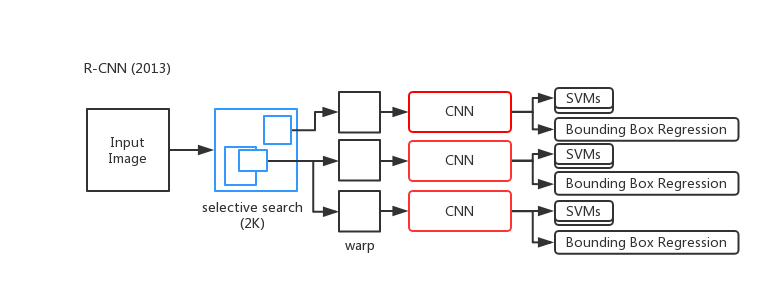
\includegraphics[width=0.9\linewidth]{figure//RCNN.png}
		\caption{R-CNN (2013) }
		\label{Fig:1}
	\end{center}
	% \vspace{-0.1em}
\end{figure}

R-CNN的缺点也是非常明显(针对于当下的算法):

\begin{itemize}
    \item region proposal的算法还是基于computer vision的selective search。
	\item 每一张图片都有将近 2K个预选区域,分别经过CNN时间开销非常庞大。
	\item warp强制转换图片的大小丢失细节。
	\item 采用SVM来分类,而针对于多个类别的时候性能远差于softmax。
\end{itemize}

\subsection{selective search}
selective search,简称为SS。是computer vision里region proposal的算法,原理是通过扫描临近的像素通过阈值的设定,来确定是否邻近的像素点是同一类。最终实现将原图分割成一块一块。这个思想和原理主要依据的是,针对于同一个物体来说颜色应该是比较相近的。

\begin{figure}[!h]
	\begin{center}
		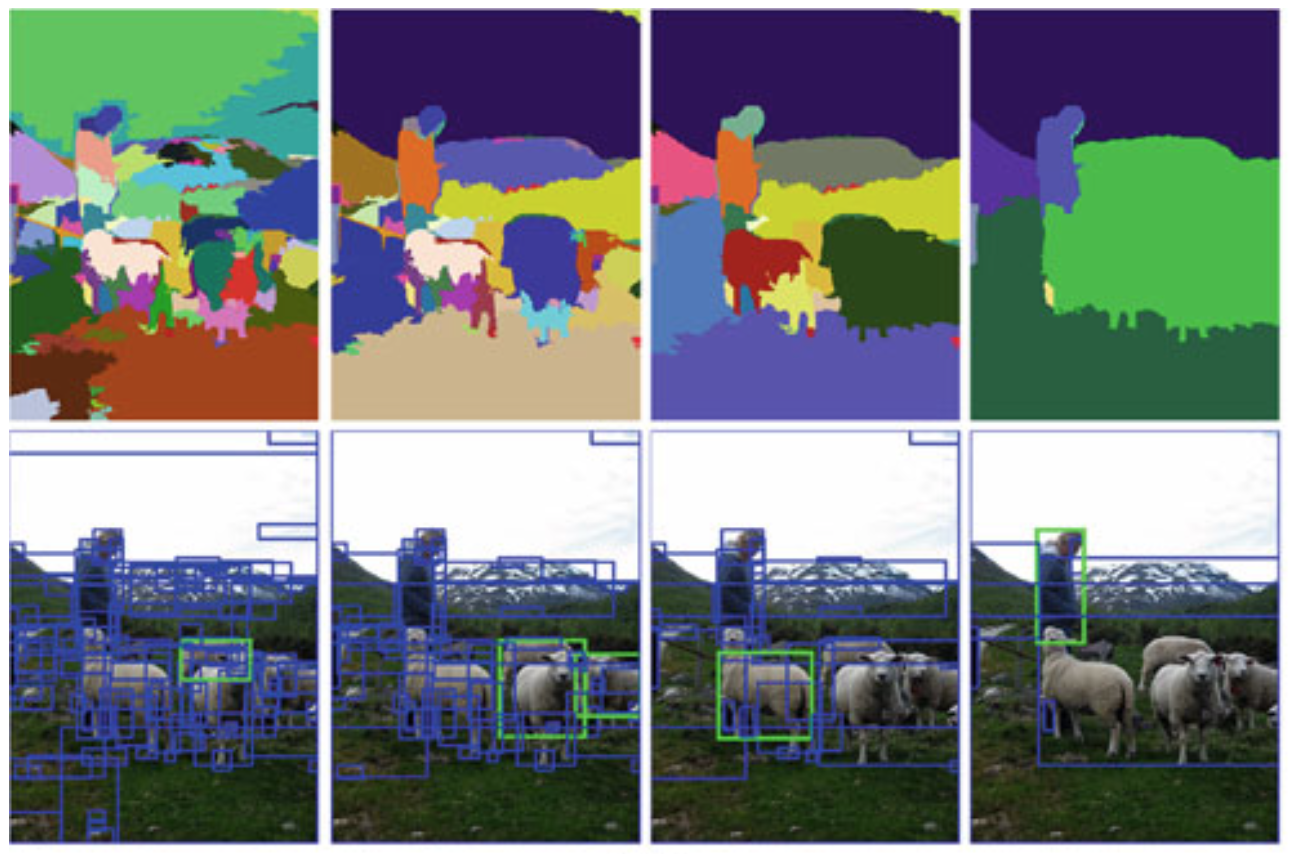
\includegraphics[width=0.92\linewidth]{figure//selectiveSearch.png}
		\caption{Selective Search }
		\label{Fig:2}
	\end{center}
	% \vspace{-0.1em}
\end{figure}


\section{SPP-net(2015.4)}

\subsection{Introduction of SPP-net(2015.4)}

其实对于R-CNN时间开销最大一处就是对于每一张图片都要经过相同CNN中,所以后人将想到CNN的共享。因为对于同一个图片针对同一个卷积和的结果是很大一部分冗余,完全可以合并后在对feature maps进行region proposal的处理。(feature maps 就是卷积后的输出,因为卷积后基本提取出图片的特征,所以取这个名字)
SPP-net就是修改了上述的这一点,并且不光如此,它还提出了取消warp,通过SPP层(Spatial Pyramid Pooling)来做到FC连接层的维度统一问题。判别分类的地方也采用了softmax改进。\\

\begin{figure}[!h]
	\begin{center}
		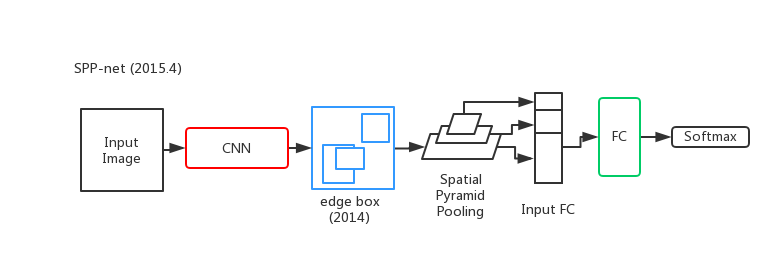
\includegraphics[width=0.92\linewidth]{figure//SPPnet.png}
		\caption{SPP-net(2015.4) }
		\label{Fig:3}
	\end{center}
	% \vspace{-0.1em}
\end{figure}

\subsection{edge box}
SPP-net采用了全新一种region proposal的算法——edge box。这算法思想是基于所有特征物体的启发式起点应该在物体的轮廓,针对于边缘轮廓的提取之后进行聚类。最终效果图如1.4所示。

\begin{figure}[!h]
	\begin{center}
		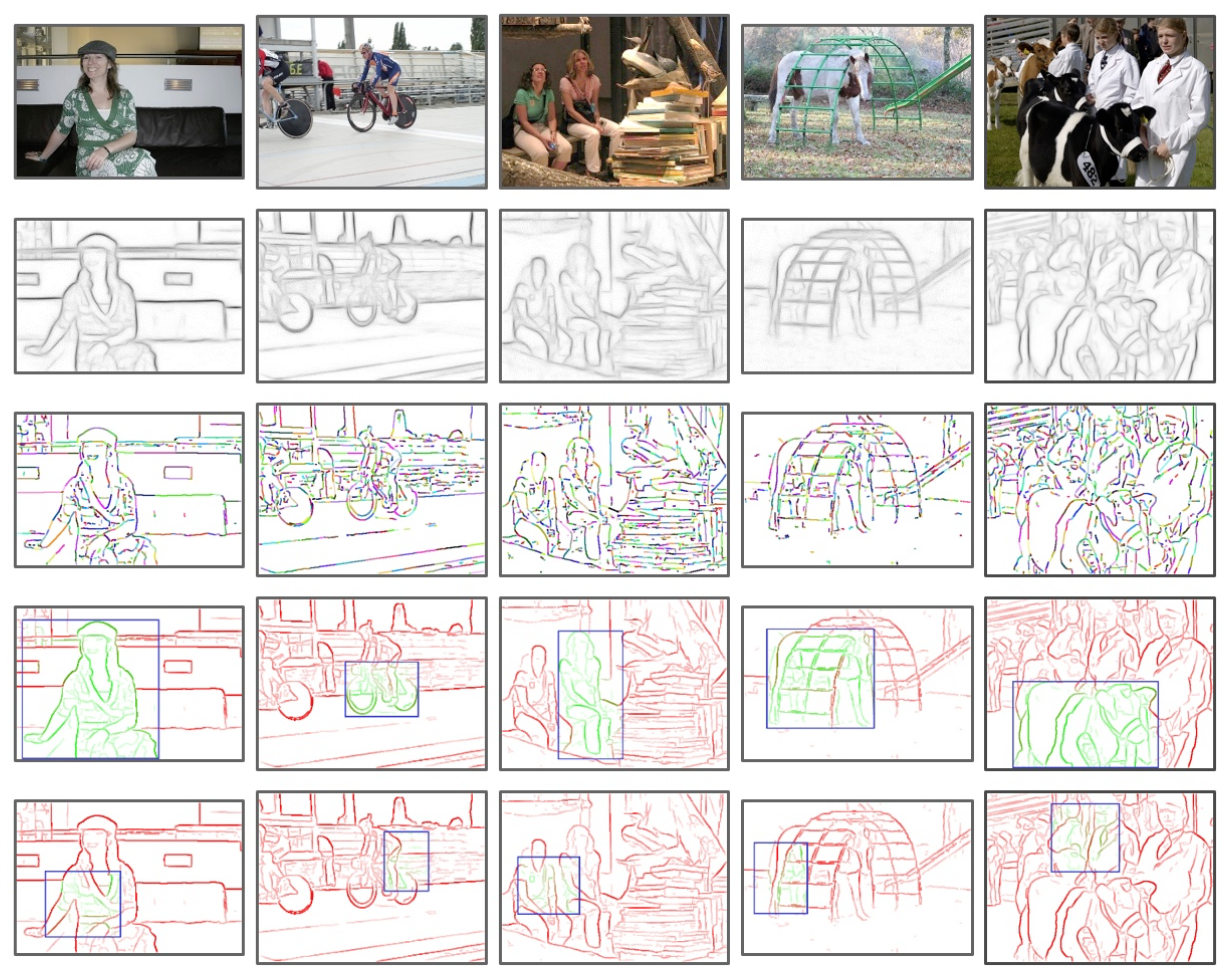
\includegraphics[width=0.7\linewidth]{figure//edgeBox.png}
		\caption{Edge Box }
		\label{Fig:4}
	\end{center}
	% \vspace{-0.1em}
\end{figure}

\section{Fast R-CNN(2015.5)}

Fast R-CNN 在region proposal的算法选择上重新选择了selective search, 在paper中作者对比了主流的方法,最终作者选择在所有数据集效果均值最好的算法(作者称为算法的稳定性)即SS(selective search)。如图1.5所示,我将SPP-net和Fast R-CNN的结构放在一起,能更加容易的发现区别。在原先SPP层(Spatial Pyramid Pooling),作者将其改成ROI(only one Pyramid level)来代替原先的三层,并且加入bounding box regression来更好的得到矩形框。

\begin{figure}[!h]
	\begin{center}
		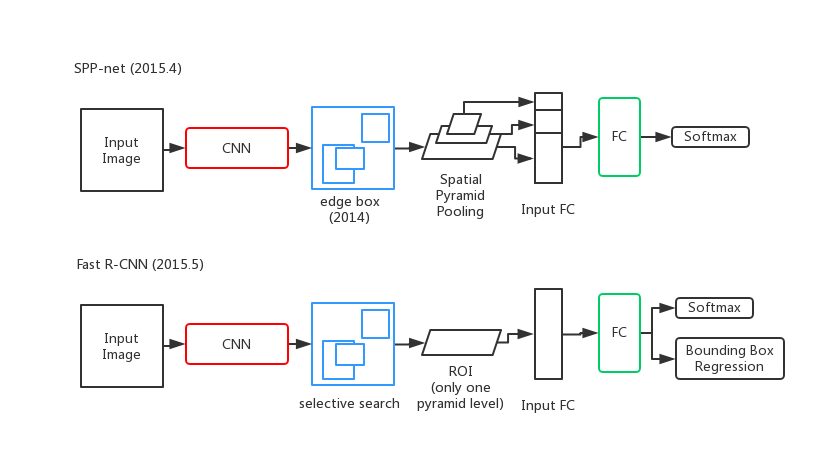
\includegraphics[width=0.92\linewidth]{figure//FastRCNN.png}
		\caption{Fast R-CNN(2015.5)}
		\label{Fig:5}
	\end{center}
	% \vspace{-0.1em}
\end{figure}

\section{Faster R-CNN(2016.1)}
Faster R-CNN 可以算R-CNN这一领域新的篇章,因为之前的算法无论如何都必须通过传统computer vision的算法来实现region proposal。这就导致在处理region proposal这算法执行无法和CNN一起放入GPU训练,使得训练时间太慢(针对于现在,之前的region proposal的算法都是在CPU上执行,速度远低于GPU)。

因此Faster R-CNN提出region proposal也可以通过神经网络来代替,作者取名为RPN(region proposal network)。在RPN中的softmax并不是类别的分类器,它只是分类是否是自己感兴趣的物体(物体与背景的二分类)。针对CNN输出的feature maps,作者提出anchor的感念。因为如果想扫描feature maps的每一块区域,我们有两种做法:1、同一大小的窗口滑动,改变输入图片的大小。2、不改变输入图片的大小,改变滑动窗口的比例和大小。很明显实验结果倾向于第二种,即作者提出anchor(就是不同大小尺寸的窗口)。在选择anchor尺寸上,在paper中是将数据集的窗口进行聚类从而选择合适的。

\begin{figure}[!h]
	\begin{center}
		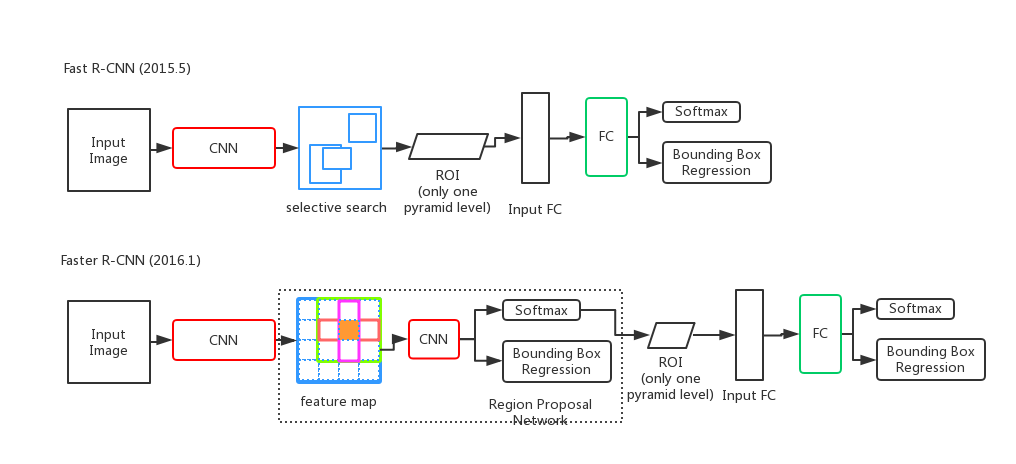
\includegraphics[width=0.92\linewidth]{figure//FasterRCNN.png}
		\caption{Faster R-CNN(2016.1)}
		\label{Fig:6}
	\end{center}
	% \vspace{-0.1em}
\end{figure}

\section{YOLO(2016.3) and SSD(2016.12) } 
在2016年期间,虽然Faster R-CNN已经取得很好的效果,但是是否还能进一步加快,或者牺牲一部分准确度提高大幅度的速度。这个目的为出发的论文就孕育而生—— YOLO(you only look once)和 SSD(single shoot detetion)。

YOLO的思想其实很简单,通过CNN将feature maps映射到原始图像,即将原始图近似看成分割成块状。这样对于feature map每个像素点直接进入全连接FC,来输出:BOOL(判别是否有物体)、bounding box的位置、类别的分类。速度效果很明显,但是缺点也很致命:1、因为feature maps像素低,所以对于细小,重叠的物体来说无法检测 2、最后使用FC代价太大。所以随后就出现YOLO-v2和YOLO9000,一部分是结构近似于SSD,改进了内部优化,如batch normalization等;另一部分word tree数据集融合的体现。(YOLO-v2和9000就一笔带过了,写起来太多了)

SSD的研究和YOLO其实是并行的,他的想法是将softmaax合二为一,这样就可以直接将Faster R-CNN的后半部分融合在一起。并且为了能检测更小的物体特征,将第一次得到的feature map在此循环进入此结构(看代码paper只执行了3次),从而在提高速度的同时也保证了精度。

\begin{figure}[!h]
	\begin{center}
		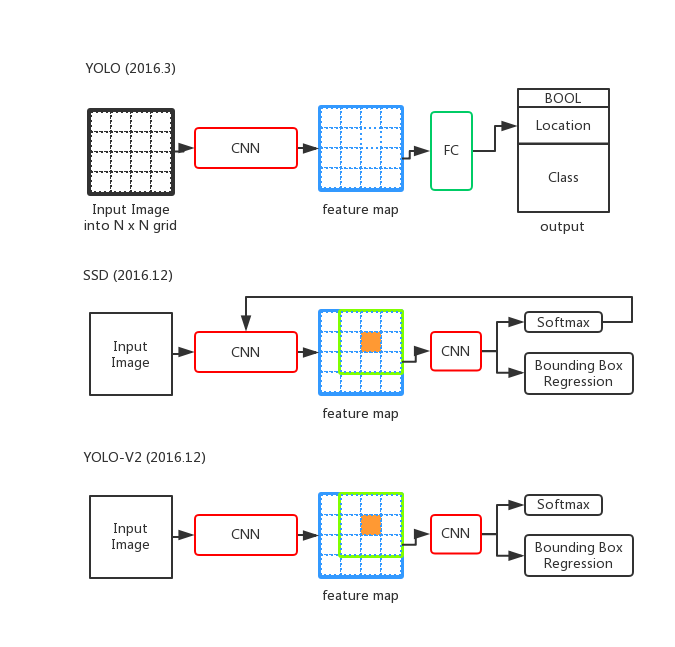
\includegraphics[width=0.92\linewidth]{figure//YOLOV2.png}
		\caption{YOLO(2016.3), SSD(2016.12) and YOLO-V2(2016.12)}
		\label{Fig:7}
	\end{center}
	% \vspace{-0.1em}
\end{figure}


\end{spacing}

%---------------------------------------------------------------------
%  
%---------------------------------------------------------------------
\chapter{Mask R-CNN}

\begin{spacing}{1.5}
\section{Introduction of Mask R-CNN(2017.4)}
Mask R-CNN从结构上看不是特别复杂,而且从算法的突破性也不是很大。但是他是第一篇将objective detection 和 Segmentation将结合在一起的论文。从图2.1所示,不难看出,Mask R-CNN的结构就是在Faster R-CNN上加入了FCN来提高模型的精确度。

\begin{figure}[!h]
	\begin{center}
		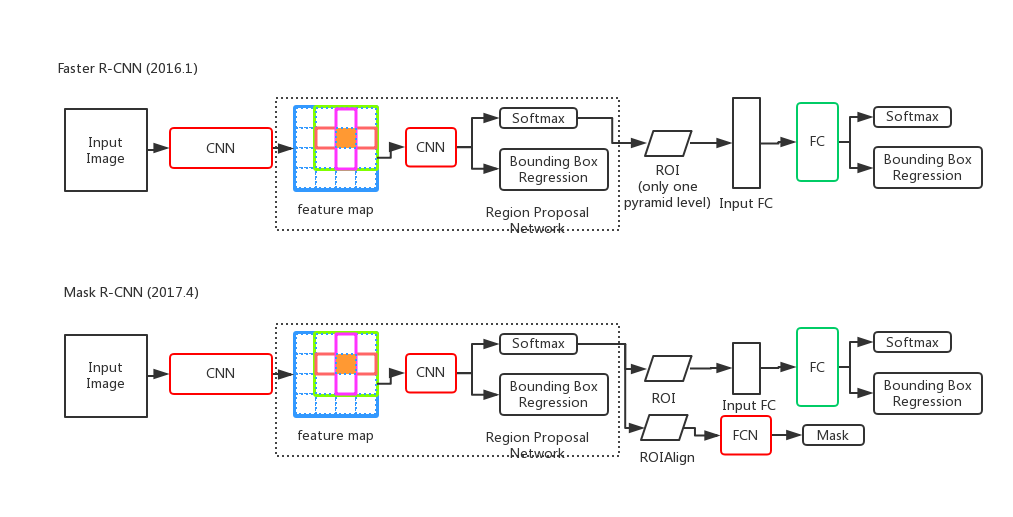
\includegraphics[width=0.92\linewidth]{figure//MaskRCNN.png}
		\caption{Mask R-CNN(2017.4)and Faster R-CNN(2016.1)}
		\label{Fig:8}
	\end{center}
	% \vspace{-0.1em}
\end{figure}

\section{ROIAlign}
这篇paper也用一种很讨巧的方法,来改进FCN得到的mask和原始图像像素直接的偏差。论文采用双向性插值的方法(先前是bounding box无需很高的精度,所以直接是按比例取整的)表达式如下。

\begin{displaymath}
  f(x ,y) = \frac{1}{(x_{2}-x_{1})(y_{2}-y_{1})}
  \left( \begin{array}{cc} x_{2}-x & x-x_{1} \end{array} \right) 
\end{displaymath}
\begin{displaymath}
  \left( \begin{array}{cc} Q_{11} & Q_{12} \\ Q_{21} & Q_{22} \end{array} \right)
  \left( \begin{array}{c} y_{2}-y \\ y-y_{1}\end{array} \right)
\end{displaymath}

另外就是用到了并行ROI的结构,来实现FCN的输入。

\section{FCN}
这部分我们组员顾天飞已经讲解,我就不多描述了。
\begin{figure}[!h]

	\centering                                             %居中
	\subfigure[]{                                          %第一张子图
	\begin{minipage}{7cm}
	\centering                                           %子图居中
	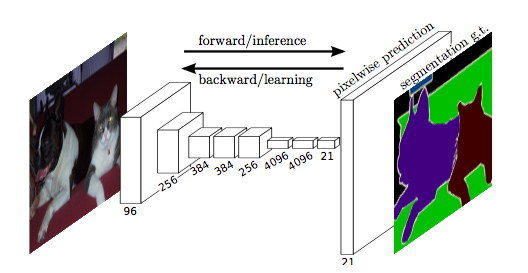
\includegraphics[scale=0.4]{figure//image10.png}             
	\end{minipage}}
	%
	%第二张子图
	\subfigure[]{                    
	\begin{minipage}{7cm}
	\centering                        %子图居中
	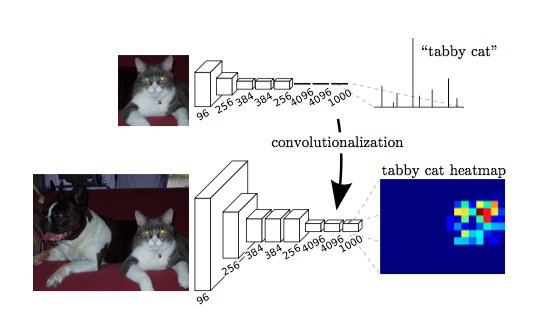
\includegraphics[scale=0.36]{figure//image11.png}             
	\end{minipage}}
	%                                           
	%大图名称
	\caption{FCN: from image to pixels} 
	\label{fig:9}                                          %图片引用标记

\end{figure}

\end{spacing}

%---------------------------------------------------------------------
%  参考文献设置
%---------------------------------------------------------------------
% \addcontentsline{toc}{chapter}{参考文献}

% \begin{thebibliography}{99}
% \songti \zihao{-4} 	
% 	\bibitem{Leslie.{1994}}
% 	Leslie Lamport. LATEX: A Document Preparation System.AddisonWesley, Reading, Massachusetts, second edition, 1994, ISBN 0-201-52983-1.
	
% 	\bibitem{Donald.{1984}}
% 	Donald E. Knuth. The TEXbook, Volume A of Computers and Typesetting,Addison Wesley, Reading, Massachusetts, second edition, 1984,ISBN 0-201-13448-9.

	
% \end{thebibliography}

%---------------------------------------------------------------------
%  附录设置
%---------------------------------------------------------------------
% \titleformat{\chapter}{\heiti\Large}{附录~\Alph{chapter}}{11pt}{\Large}
% \titlespacing{\chapter}{0pt}{*-4}{*4}

% \lstset{breaklines}                %自动将长的代码行换行排版
% \lstset{extendedchars=false}
% \lstset{language=Matlab}
% \renewcommand{\thechapter}{附录\Alph{chapter}.} 
% \appendix
% \begin{appendix}
	
	
% \chapter{数据表}
% \zihao{-4}\songti
% \begin{spacing}{1.5}
% 	hello world!
% \end{spacing}


% \chapter{程序代码}
% \zihao{-4}\songti
% \begin{spacing}{1.5}
% 下面是一个MATLAB程序的事例,使用了Package mcode,它能较好还原MATLAB本身的编写风格。
% \begin{lstlisting}
% %The program normalizes the measurement data and compares it to the standard cosine function
% data=xlsread('data_sun',1,'B3:E39');
% min=[(data(1,1)+data(37,1))/2,(data(1,2)+data(37,2))/2,...
% (data(1,3)+data(37,3))/2,(data(1,4)+data(37,4))/2];
% max=[data(19,1),data(19,2),data(19,3),data(19,4)];
% Min=repmat(min,37,1);
% Max=repmat(max,37,1);
% data=(data-Min)./(Max-Min);
% x=-pi/2:pi/36:pi/2;
% y=cos(x);
% %----------------------figure-------------------------%
% figure(1);
% subplot(2,2,1);
% plot(x,data(:,1),'ro-');
% hold on;
% plot(x,y,'b-');
% title('R=1.2\Omega');
% axis([-2,2,0,1]);
% grid on;
% subplot(2,2,2);
% plot(x,data(:,2),'ro-');
% hold on;
% plot(x,y,'b-');
% title('R=1.6\Omega');
% axis([-2,2,0,1]);
% grid on;
% subplot(2,2,3);
% plot(x,data(:,2),'ro-');
% hold on;
% plot(x,y,'b-');
% title('R=2.0\Omega');
% axis([-2,2,0,1]);
% grid on;
% subplot(2,2,4);
% plot(x,data(:,4),'ro-');
% hold on;
% plot(x,y,'b-');
% title('R=2.4\Omega');
% grid on;
% axis([-2,2,0,1]);
% \end{lstlisting}
% \end{spacing}
% \end{appendix}
		

\end{document}
